
\chapter{Stand der Technik}\label{chap:Stand_der_Technik}
\section{Datenverarbeitungskette}

Die Datenerhebung findet über eine Polysomnographie im Schlaflabor statt. Richtlinien dazu finden sich in der \cite{AASM}. In einer Standarduntersuchung werden ein Elektroenzephalogramm (EEG), ein Elektrookulogramm und Elektromyogramme (EMG) erstellt \cite{1x1}. Das EMG besteht aus den Elektroden, einer Verstärkerschaltung, einem Analog-Digital-Umsetzer und Filtern \cite{biomechanist} \cite{PRT}. Der Analog-Digital-Umsetzer soll mit mindestens 200 Hertz (möglichst mit 500 Hertz) und einer 12 Bit Quantisierung arbeiten \cite{AASM}. Üblich sind heutzutage 16 bis 22 Bit \cite{SleepDisordersMedicine}.

Außerdem können bei Bedarf 50 Hz beziehungsweise 60 Hz (in Amerika) Notchfilter eingesetzt werden. Die AASM rät davon allerdings ab, da die Aufzeichnung der Muskelaktivität beeinträchtigt werden könnte \cite{PRT}.
Der Start der eigentlichen Messung beginnt mit dem Löschen des Lichtes (Licht aus) und endet mit dem Anschalten des Lichtes (Licht an) \cite{1x1}. Die Aufzeichnung wird auf den Monitoren mit einer Geschwindigkeit von zehn Millimeter pro Sekunde dargestellt, sodass auf einen Bildschirm 30 Sekunden passen \cite{PRT}. Die Einteilung ist historisch aus den Aufzeichnungen auf Endlospapier entstanden, welches nach 30 Sekunden umklappte. Die gesammelten Daten werden anschließend verwendet, um unter anderem motorische, respiratorische und EEG-bezogene Ereignisse zu finden und zu klassifizieren. \cite{PDS}

Die Software der Aufzeichnungsgeräte verfügt meistens direkt über eine Annotationsunterstützung, welche Vorschläge für die Start- und Endzeitpunkte der Beinbewegungen (LM) macht. Diese werden vom Assistenzpersonal überarbeitet. Vorschläge, die mit atembezogenen Events (zum Beispiel einer Schlafapnoe) zusammenhängen, sollen laut AASM gelöscht werden. Abschließend werden Regeln zur Bestimmung von periodischen Beinbewegungen angewandt (siehe Kapitel: „medizinische Grundlagen“), um die PLMS-Kennwerte zu bestimmen (Anzahl von PLMS, Anzahl von PLMS mit Arousals, PLMS-Index, PLMS-Arousal-Index) \cite{Carvelli}. Die Annotationen werden später von einem Somnologen oder von einem Arzt für Schlafmedizin überprüft \cite{PDS}. \cite{PRT}

In dem Prozessbild \ref{fig:Prozessbild} ist die Datenverarbeitungskette dargestellt. Als Eingangssignal auf der linken Seite ist das EMG Signal aus dem Schlaflabor zu sehen, welches durch das medizinische Personal -meist mithilfe der Annotationsunterstützung- auf Beinbewegungen untersucht wird. Durch die Verarbeitung entsteht ein binäres Annotationssignal, welches jedem Zeitpunkt aus dem ursprünglichen EMG-Signal zuweist, ob an diesem Zeitpunkt eine Beinbewegung vorliegt oder nicht. Anhand dieses Annotationssignals wendet ein Algorithmus die Kriterien der AASM an und berechnet Kennwerte, die repräsentativ für das Annotationssignal stehen.


\begin{figure}[!ht]%
	\begin{center}
	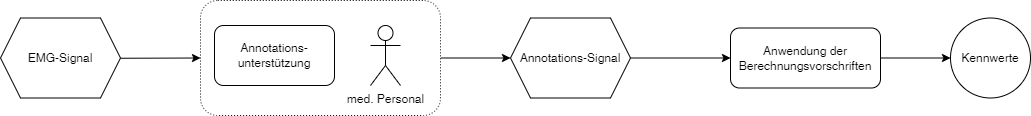
\includegraphics[width=0.80\textwidth]{./Bilder/Prozessbildrot.drawio.png}
	\end{center}
	\caption{Veranschaulichung der Datenverarbeitungskette. Das EMG-Signal wird von medizinischem Personal mithilfe von Annotationsunterstützung verarbeitet. Rechts im Bild sind die Kennwerte dargestellt, die von einem Algorithmus berechnet werden und das Ergebnis der Kette beschreiben.}%
	\label{fig:Prozessbild}%
\end{figure}

\section{Detektoren}
Die Detektoren können nach der Art der Vorverarbeitung der Eingangsdaten, der Merkmalsextraktion und der Klassifizierung unterschieden werden. Es gibt sehr unterschiedliche Möglichkeiten die Merkmalsextraktion umzusetzen. Sie kann beispielsweise im Frequenzbereich (spektrale Kantenfrequenz\footnote{Frequenz unter der ein bestimmter Prozentsatz der Gesamtleistung liegt.}, fraktaler Exponent\footnote{Maß für Signalkomplexität: Steigung der Geraden in der doppeltlogarithmischen Darstellung spektrale Leistungsdichte gegen Frequenz \cite{dirichlet}.}) \cite{dirichlet}, im Zeit-Frequenzbereich (Waveletkoeffizienten) \cite{shroko} oder im Zeitbereich (Spikewiederholrate, durchschnittliche Amplitude, Länge des Zeitfensters in dem Spikes auftreten) \cite{wetter} stattfinden. Die Auswertung kann zum Beispiel über statistische Klassifikatoren \cite{probabilistic,dirichlet} oder Neuronale Netze \cite{Carvelli,shroko} erfolgen.

Am meisten verbreitet sind die Detektoren, die im Zeitbereich eine Schwellwertklassifikation mit einem absoluten \cite{wetter,ferri,Huang,stefani,tauchmann} oder dynamischen \cite{alvarez,Moore} Schwellwert vornehmen. Hierbei wird meist die Amplitude des vorverarbeiteten Signals als Merkmal genutzt. Der Detektor von Carvelli et al. nutzt ein \gls{DNN} für die Klassifikation.

Für ein besseres Verständnis der Funktionsweise wird im Folgenden der Algorithmus von Moore et al. zusammengefasst. Dieser wurde gewählt, da der Ansatz weit verbreitet ist und Ideen von Tauchmann, Ferri et al. und Wetter et al. aufgegriffen und weiterentwickelt wurden. 


\begin{enumerate}
	\item Einlesen des Datensatzes
	
	Die beiden EMG-Signale der Beine werden zu einem Signal zusammengeführt und die Elektrokardiogrammstörung mithilfe eines adaptiven Filters vermindert.
    Das gesäuberte Signal wird gleichgerichtet zu x(n).
    Für die Annotation wird das RMS y(n) von x(n) mit einem beidseitigem 0.15-sekündigen Fenster gebildet. 

	\item Berechnung des Grundrauschens
	
	Aus dem x(n) wird mithilfe eines 20-sekündigen gleitenden Mittelwertes das vorläufige Grundrauschen $\eta$ (n) ermittelt. Das Grundrauschsignal ist nur vorläufig, da alle Beinbewegungen mit in den Mittelwert eingerechnet werden und somit fälschlicherweise das Grundrauschen erhöhen. 
    Aus dem Grundrauschen wird auch der vorläufige erste und zweite Schwellwert berechnet ($\alpha$ und $\beta$)
    \[ \alpha(n) = \left\{\begin{matrix}\eta(n)\log(\eta(n)+1)+U \\\infty \end{matrix}
    \right.\begin{matrix}, \eta\leq 50\\, \eta> 50
    \end{matrix}\]
    \[ \beta(n) = \frac{L}{U} \alpha(n) \]


    \item Berechnung der Annotation
        
    Diese Schwellwerte weichen bewusst von den definierten Werten der AASM Kriterien ab, orientieren sich jedoch an diesen durch die Startwerte L und U. Der Startzeitpunkt für einen Beinbewegungskandidaten ist der Zeitpunkt, bei dem y(n) das erste Mal den oberen Schwellwert überschreitet. Die Beinbewegung endet, wenn das RMS-Signal für 0.05 Sekunden unter dem unteren Schwellwert bleibt. Kandidaten, die weniger als 0.1 Sekunden voneinander trennt, werden zusammengefasst. 
    Um den Verlauf des Grundrauschens besser zu approximieren, wird an den Stellen, an denen Beinbewegungenskandidaten erkannt wurden, der Wert des absoluten EMG-Signals auf die Hälfte des zweiten Schwellwertes $\beta$(n) gesetzt. Dieses Signal ist das finale Grundrauschen.
    
\end{enumerate}



\section{Klassische Metriken}



Die Metriken können segmentweise oder eventweise berechnet werden. Ein Segment wird meist als positiv gezählt, wenn das binäre quasizeitkontinuierliche Signal bei mehr als 50\% des Segmentzeitraumes positiv ist. Wenn die Segmente die Länge eines Abtastzeitraumes haben, geht die segmentweise Klassifikation in eine sampleweise Klassifikation über.
Bei der eventweisen Klassifikation erfolgt die Zuordnung analog. Hier wird jedoch meistens (mit Ausnahme von \cite{stefani}) ein TP gezählt, sobald sich die beiden Annotationszeiträume mit mindestens einem Abtastwert überlappen. Dabei kann es passieren, dass mehrere Events in einem Signal auftreten, während in der anderen Annotation nur ein Event gefunden wurde. Hier findet eine multiple Zuordnung statt, bei der für alle dieser Events ein TP gezählt wird. Die Notation ist analog zu Wetter et al. mit Xto1-Matching bei mehreren manuellen Annotationen und 1toX-Matching bei mehreren automatischen Annotationen.

Die Abbildung \ref{fig:Zuordnung} gibt einen Überblick über die segmentweise und eventweise Klassifikation zusammen. Zu beachten ist, dass die Events in der Auswertung nicht mit ihrer Zeit gewichtet werden, sondern nur gezählt werden. 

\begin{figure}[!ht]%
	\begin{center}
	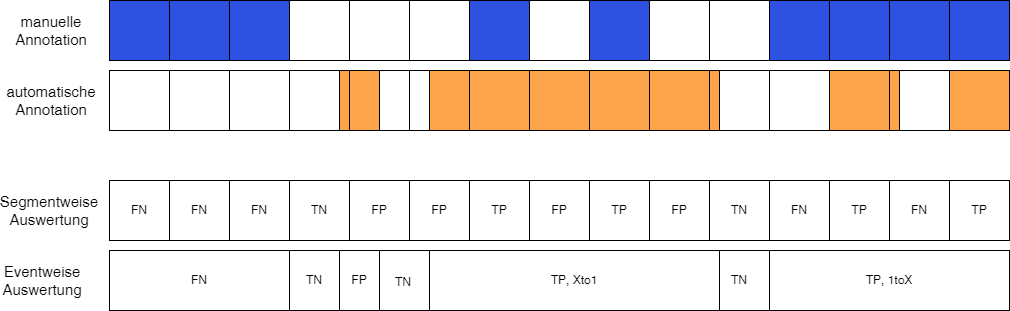
\includegraphics[width=0.80\textwidth]{./Bilder/Zuordnung.png}
	\end{center}
	\caption{Klassifizierung von \gls{TP}, \gls{TN}, \gls{FP} und \gls{FN} nach segement- und eventweiser Berechnung bei segemtierter manueller und quasizeitkontinuierlicher automatischer Annoatation.}%
	\label{fig:Zuordnung}%
\end{figure}

Die wichtigsten klassischen Metriken aus der Literatur werden im Folgenden vorgestellt.\\

\noindent\textbf{\gls{rr} (PLM/h)}\\ 
\begin{equation}\frac{ \sum_{i=1}^{n} (x_i - \Bar{x})(y_i - \Bar{y})}{\sqrt{\sum_{i=1}^{n} (x_i - \Bar{x})^{2}} \sqrt{\sum_{i=1}^{n} (y_i - \Bar{y})^{2}}}\end{equation}\\
\textbf{Cohens $\kappa$}\\
\begin{equation}
P_e = \frac{(TP+FN)(TP+FP)+(TN+FP)(TN+FN)}{(TP+TN+FP+FN)^{2}}\\\end{equation}
\begin{equation}P_0 = \frac{TP+TN}{2}\\\end{equation}
\begin{equation}\kappa = \frac{P_0 - P_e}{1-P_e}\\\end{equation}
\textbf{F1-Ma"s}\\
\begin{equation}\frac{2TP}{2TP+FP+FN}\\\end{equation}
\textbf{AUROC}\\
Integral unter der Grenzwertoptimierungskurve beim Verändern des Entscheidungsschwellwertes\\
\textbf{AUPRC}\\
Integral unter der Genauigkeits-Sensititvitäts-Kurve beim Verändern des Entscheidungsschwellwertes\\
\textbf{\gls{Prec}}\\
\begin{equation}\frac{TP}{TP+FP}\\\end{equation}
\textbf{\gls{NPV}}\\
\begin{equation}\frac{TN}{TN+FN}\\\end{equation}
\textbf{\gls{Acc}}\\
\begin{equation}\frac{TP+TN}{TP+TN+FP+FN}\\\end{equation}
\newpage
\noindent
\textbf{\gls{Sens}}\\
\begin{equation}\frac{TP}{TP+FN}\\\end{equation}
\textbf{\gls{Spez}}\\
\begin{equation}\frac{TN}{TN+FP}\\\end{equation}
\textbf{\gls{FPrate}}\\
\begin{equation}\frac{FP}{FP+TP}\\\end{equation}


Die Tabellen \ref{tab:Stand der Technik1} und \ref{tab:Stand der Technik2} beschreiben den Stand der Technik und geben einen Überblick welche Detektoren aus der Literatur bereits welche Ergebnisse erzielen konnten.

\begin{table}[!ht]
    \caption{Stand der Technik, Teil 1; Der Zusatz 'r' bezeichnet einen rekonstruierten Wert}   
	\centering
		\begin{tabular}{llllllllll}
			\hline & \cite{Huang} & \cite{Moore} & \cite{Moore} & \cite{alvarez} & \cite{ferri}\\
			\hline {$\!\begin{aligned}
				&\\
			    Datensatz\\
			    Art\ des\ Klassifikators\\
			    Berechnungsart\\
			    \gls{Sens}\\
			    \gls{Prec}\\
			    \gls{Spez}\\
			    \gls{NPV}\\
			    \gls{Acc}\\
			    Cohens\ \kappa\\
			    F1-Ma"s\\
			    Korrealtion\ PLM/h\\
			    relative\ \#\ PLM\\
				&\\
				\end{aligned}$} & {$\!\begin{aligned}
				&\\
				15\ \gls{RLS}\ (24)\\
				statisch\\
				Event\\
				0.95\\
				-\\
				0.92\\
				-\\
				-\\
				-\\
				0.93r\\
				0.97\\
				1.05\\
				&\\
				\end{aligned}$} & {$\!\begin{aligned}
				&\\
				\acrshort{WSC}\ (1073)\\
				dynamisch\\
			    Event\ \cite{git}\\
				0.6\\
				0.88\\
				1\\
				0.99\\
				0.98\\
				0.71\\
				-\\
				0.94\\
				0.63\\
				&\\
				\end{aligned}$} & {$\!\begin{aligned}
				&\\
				\acrshort{SSC}\ (760)\\
				dynamisch\\
				Event\ \cite{git}\\
				0.75\\
				0.82\\
				1\\
				0.99\\
				0.99\\
				0.87\\
				-\\
				0.94\\
				0.92\\
				&\\
				\end{aligned}$}  & {$\!\begin{aligned}
				&\\
			    \acrshort{HMC}\ (70)\\
				dynamisch\\
				Segment\ (1s)\\
				0.82\\
				0.71\\
				1\\
				-\\
				1\\
				0.73\\
				0.73\\
				-\\
				0.99\\
				&\\
				\end{aligned}$}  & {$\!\begin{aligned}
				&\\
				\acrshort{WSC}\ (60)\\
				statisch\\
				Event\\
				0.85\\
				0.62\\
				0.99\\
				1\\
				0.99\\
				0.72\\
				-\\
				-\\
				1.33\\
				&\\
				\end{aligned}$}
				\\
				\hline
		\end{tabular}

\label{tab:Stand der Technik1}
\end{table}

\begin{table}[!ht]
    \caption{Stand der Technik, Teil 2}   
	\centering
		\begin{tabular}{llllllllll}
			\hline & \cite{wetter} & \cite{Carvelli}& \cite{Carvelli}& \cite{Carvelli}\\
			\hline {$\!\begin{aligned}
			    &\\
			    Datensatz\\
			    Art\ des\ Klassifikators\\
			    Berechnungsart\\
			    \gls{Sens}\\
			    \gls{Prec}\\
			    \gls{Spez}\\
			    \gls{NPV}\\
			    \gls{Acc}\\
			    Cohens\ \kappa\\
			    F1-Ma"s\\
			    Korrealtion\ PLM/h\\
			    relative\ \#\ PLM\\
				&\\
				\end{aligned}$} & {$\!\begin{aligned}
				&\\
				\acrshort{WSC}\ (60)\\
				statisch\\
				Event\\
				0.96\\
				0.47\\
				0.98\\
				1\\
				0.98\\
				0.62\\
				-\\
				-\\
				2.05\\
				&\\
				\end{aligned}$} & {$\!\begin{aligned}
				&\\
                \acrshort{WSC}\ (275)\\
				\acrshort{DNN}\\
				Event\\
				0.9\\
				0.81\\
				-\\
				-\\
				-\\
				-\\
				0.83\\
				-\\
				-\\
				&\\
				\end{aligned}$}& {$\!\begin{aligned}
				&\\
                \acrshort{SSC}\ (177)\\
				\acrshort{DNN}\\
				Event\\
				-\\
				-\\
				-\\
				-\\
				-\\
				-\\
				0.71\\
				-\\
				-\\
				&\\
				\end{aligned}$}& {$\!\begin{aligned}
				&\\
                MrOS\ Sleep\ Study\ (348)\\
				\acrshort{DNN}\\
				Event\\
				-\\
				-\\
				-\\
				-\\
				-\\
				-\\
				0.77\\
				-\\
				-\\
				&\\
				\end{aligned}$}
				\\
				\hline
		\end{tabular}

\label{tab:Stand der Technik2}
\end{table}


Bei der eventweisen Berechnungsart wurde ein TP bei jeglicher Überlappung gewertet. Die Werte für den Detektor von Wetter et al. sind aus \cite{Moore} übernommen.
Der Zahlenzusatz 'r' steht dafür, dass dieser Wert nicht veröffentlicht wurde, aber aus den anderen Metriken rekonstruiert werden konnte.
Die Zahl in Klammern am Ende der Datensatzbeschreibung bezeichnet die Gesamtanzahl der Patienten im verwendeten Datensatz.